% --- SEZIONE 3: ARCHITETTURE E COMPILAZIONE ---

\section{Confronto Architetture ARM Cortex}
\begin{description}
    \item[Cortex-A (Application):] Generische Berechnung mit hoher Leistung (Linux/Android).
    \item[Cortex-R (Real-Time):] Geringe Latenz und hohe Zuverlässigkeit (Automotive/Medizin).
    \item[Cortex-M (Microcontroller):] Reduzierter Energieverbrauch, deterministische Interrupts.
\end{description}

\renewcommand{\arraystretch}{1.5}
\resizebox{\columnwidth}{!}{
\begin{tabular}{|l|c|c|c|c|c|c|c|c|}
\hline
\textbf{Core} & \textbf{Thumb} & \textbf{Thumb-2} & \textbf{HW Mult.} & \textbf{HW Div.} & \textbf{Math Sat.} & \textbf{DSP} & \textbf{FPU} & \textbf{Arch} \\
\hline
Cortex-M0  & \cellcolor{green!60}Mostly & \cellcolor{green!60}Subset & \cellcolor{green!60}1/32 cyc & \cellcolor{red!60}No & \cellcolor{red!60}No & \cellcolor{red!60}No & \cellcolor{red!60}No & ARMv6-M \\
Cortex-M0+ & \cellcolor{green!60}Mostly & \cellcolor{green!60}Subset & \cellcolor{green!60}1/32 cyc & \cellcolor{red!60}No & \cellcolor{red!60}No & \cellcolor{red!60}No & \cellcolor{red!60}No & ARMv6-M \\
Cortex-M1  & \cellcolor{green!60}Mostly & \cellcolor{green!60}Subset & \cellcolor{green!60}3/33 cyc & \cellcolor{red!60}No & \cellcolor{red!60}No & \cellcolor{red!60}No & \cellcolor{red!60}No & ARMv6-M \\
Cortex-M3  & \cellcolor{green!60}Fully  & \cellcolor{green!60}Fully  & \cellcolor{green!60}1 cyc    & \cellcolor{green!60}Yes & \cellcolor{green!60}Yes & \cellcolor{red!60}No  & \cellcolor{red!60}No & ARMv7-M \\
Cortex-M4  & \cellcolor{green!60}Fully  & \cellcolor{green!60}Fully  & \cellcolor{green!60}1 cyc    & \cellcolor{green!60}Yes & \cellcolor{green!60}Yes & \cellcolor{green!60}Yes & \cellcolor{yellow!60}Optional & ARMv7E-M \\
Cortex-M7  & \cellcolor{green!60}Fully  & \cellcolor{green!60}Fully  & \cellcolor{green!60}1 cyc    & \cellcolor{green!60}Yes & \cellcolor{green!60}Yes & \cellcolor{green!60}Yes & \cellcolor{yellow!60}Optional & ARMv7E-M \\
\hline
\end{tabular}}
\renewcommand{\arraystretch}{1}

\subsection{Evoluzione Cortex-M0 vs M0+}
\begin{minipage}[t]{0.49\columnwidth}
    \begin{itemize}
        \item \textbf{M0+ Pipeline:} Auf 2 Stufen reduziert für höhere Effizienz.
        \item \textbf{I/O-Zugriff:} Unterstützung für Single-Cycle GPIO.
        \item \textbf{Debugging:} Optionaler Micro Trace Buffer (MTB) zum Nachverfolgen von Sprüngen.
        \item \textbf{MPU}
    \end{itemize}
\end{minipage}\hfill
\begin{minipage}[t]{0.49\columnwidth}
    \textbf{Pipeline}
    \begin{itemize}
        \item[+] Es wird in jedem Cycle ein Befehl ausgeführt
        \item [-] Bei Sprüngen muss die Pipeline 'geleert' werden
    \end{itemize}
\end{minipage}


\section{Adressierungsarten ARM (Cortex-M0)}
\begin{minipage}{0.5\columnwidth}
    \begin{itemize}
        \item Register direkt
        \item Register Indirekt
    \end{itemize}
\end{minipage}
\begin{minipage}{0.5\columnwidth}
    \begin{itemize}
        \item Register Indirekt mit offset \texttt{[R?, \#imm]}
        \item Register Indirekt mit index \texttt{[R?, R?]}
    \end{itemize}
\end{minipage}

\begin{minipage}[t]{0.5\columnwidth}
    \subsection{Register Direkt, Immediate}
    \begin{itemize}
        \item \textbf{Immediate:} \texttt{MOV R0, \#100} $\rightarrow$ Der Wert wird direkt geladen.
        \item \textbf{Register:} \texttt{MOVS R2, R1} $\rightarrow$ Kopiert den Wert zwischen Registern.
        \item \textbf{Einschränkungen:} Die Immediate-Werte werden in der Instruktion kodiert (z.B. 8-bit für \texttt{MOVS}).
    \end{itemize}

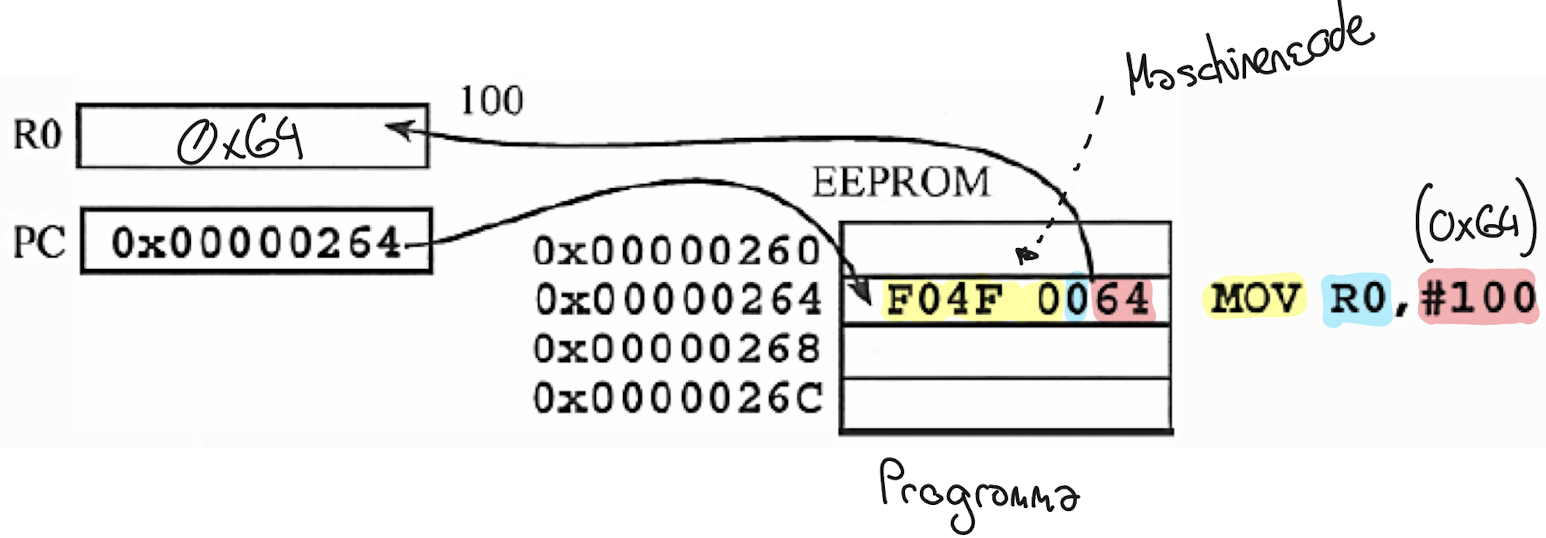
\includegraphics[width=\linewidth]{images/register_direkt.png}
\end{minipage}
\begin{minipage}[t]{0.5\columnwidth}
    \subsection{Register Indirekt (ptr)}
    \begin{itemize}
        \item \textbf{Einfach:} \texttt{LDR R0, [R1]} \\
        $\rightarrow$ $R0 = \text{Wert an der Adresse } R1$.
        \item \textbf{Mit Offset:} \texttt{LDR R0, [R1, \#4]} $\rightarrow$ $R0 = \text{Wert an der Adresse } R1 + 4$ (nützlich für Arrays/Structs).
        \item \textbf{Mit Index:} \texttt{LDR R0, [R1, R2]} \\
        $\rightarrow$ $R0 = \text{Wert an der Adresse } R1 + R2$.
    \end{itemize}    
    \begin{center}
        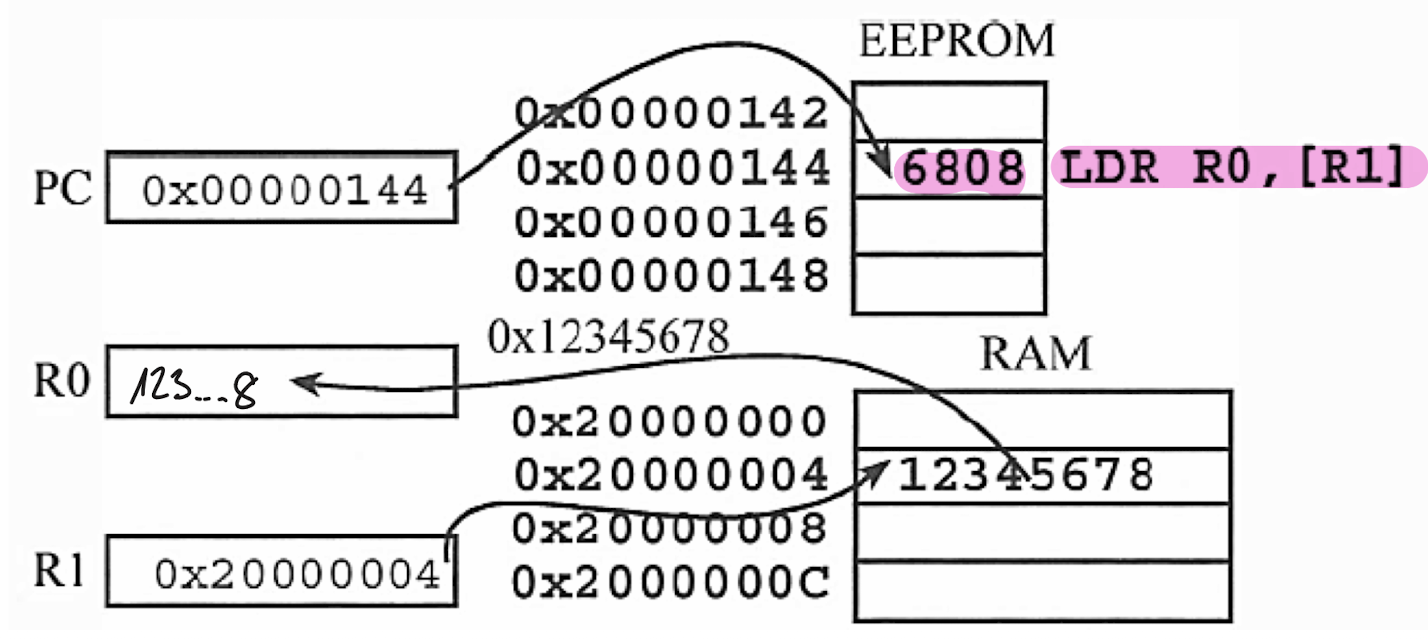
\includegraphics[width=\linewidth]{images/register_indirekt.png}
    \end{center}
\end{minipage}

\subsection{PC-Relative \& Literal Pool}
\begin{itemize}
    \item \textbf{Problem:} 32-bit-Instruktionen können keine 32-bit-Konstanten enthalten.
    \item \textbf{Lösung:} Der Assembler speichert die Konstante im \textbf{Literal Pool} (Speicherbereich in der Nähe).
    \item \textbf{Zugriff:} \texttt{LDR R0, =0x12345678} wird übersetzt in \texttt{LDR R0, [PC, \#offset]}.
    \item Es sind immer \textbf{zwei Speicherzugriffe} erforderlich
\end{itemize}

\subsection{Registerlisten \& Stack (SP-Relative)}
\begin{itemize}
    \item \textbf{Multiple:} \texttt{LDM R7!, \{R0-R3, R5\}} $\rightarrow$ Lädt mehrere Register beginnend bei der Adresse in $R7$.
    \item \textbf{Stack:} \texttt{PUSH \{R0-R2\}}, \texttt{POP \{R0-R2\}}.
    \item \textbf{Goldene Regel:} Das Register mit der niedrigsten Nummer (\texttt{R0}) geht immer in die niedrigste Speicheradresse. Die Reihenfolge in den geschweiften Klammern ist für die Hardware nicht relevant.
\end{itemize}

\subsection{Stack Framing}
Der Stack Frame ist der in RAM reservierte Bereich für lokale Variablen einer Funktion.

\begin{minipage}{0.5\columnwidth}
    \begin{itemize}
        \item \textbf{Allokation:} \texttt{SUB SP, SP, \#X} reserviert $X$ Byte (der Stack wächst zu niedrigeren Adressen).
        \item \textbf{Frame Pointer ($R7$):} Man verwendet \texttt{MOV R7, SP}, um einen festen Bezug zum Anfang des Frames zu haben.
        \item \textbf{Zugriff:} Die Variablen werden unter Verwendung von Offsets relativ zu $R7$ geschrieben/gelesen, z.B.: \texttt{STR R0, [R7, \#4]}.
        \item \textbf{Deallokation:} Vor dem Rücksprung (\texttt{BX LR}) muss der Stack mit \texttt{ADD SP, SP, \#X} bereinigt werden.
    \end{itemize}
\end{minipage}
\begin{minipage}{0.5\columnwidth}
    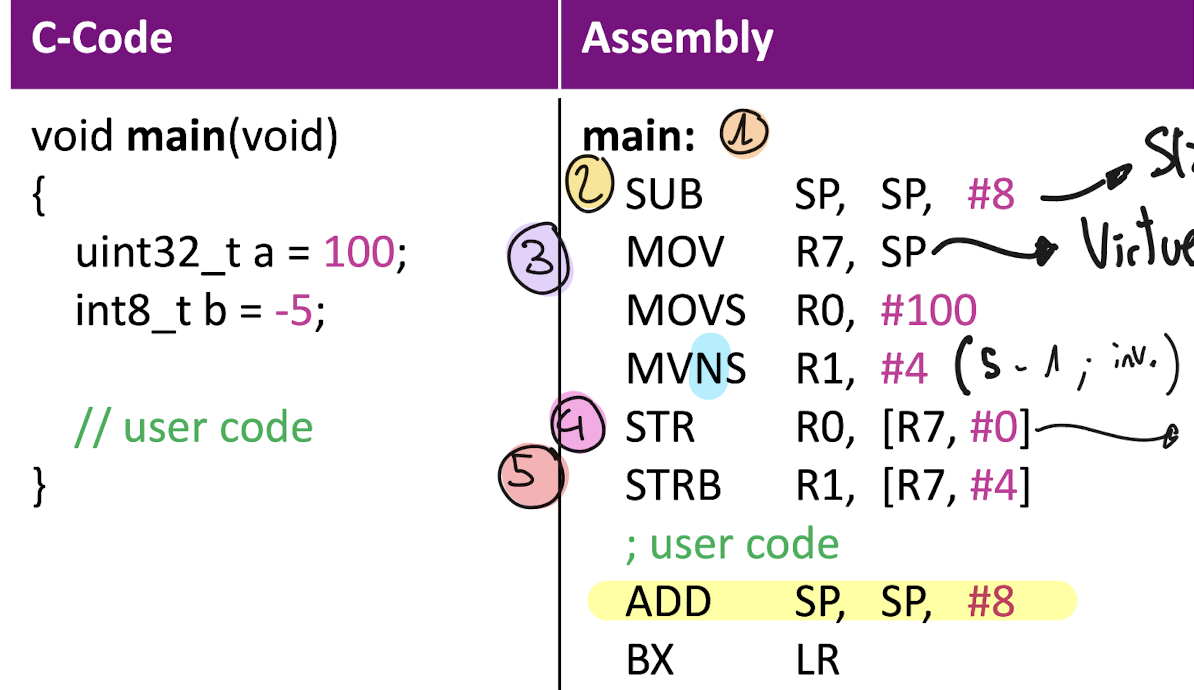
\includegraphics[width=\linewidth]{images/stack_framing.png}
\end{minipage}

